\section{Limit plots}

\subsection{ggF and VBF Channel Combination}

The observed (expected) upper limit on the SM ggF+VBF signal strength, including the cross section uncertainty from theory calculations, is 5.45 (8.09) and shown in Table \ref{table:ggfvbf-sm-xs-tab}. The limit set on \kl using the combined ggF and VBF channels are the strongest constraints set on this coupling in the \bbbb final state in ATLAS to date. 

Expected and observed upper limits on the ggF+VBF cross section are $7.36 \times 32.776 = 241.20$ $5.02 \times 32.776 = 164.49$, where the theory calculation uncertainties on the ggF and VBF cross sections are excluded.

\begin{table}[h]
	\centering
	\caption{The observed and expected upper limit on the SM \HH production cross-section at the 95\% CL. The expected value is shown with corresponding one and two standard deviation error bounds.}
	\begin{tabular}{c c c c c c c}
		\toprule
		{} & {Observed} & {$-2\sigma$} & {$-1\sigma$} & {Expected} & {$+1\sigma$} & {$+2\sigma$}\\
		\midrule
		{ggF production: ggF channel fit} & {5.73}  & {4.44} & {5.97} & {8.28} & {12.51} & {19.71}  \\
		{ggF production: ggF+VBF channels fit} & {5.51}  & {4.41} & {5.92} & {8.22} & {12.43} & {19.62}  \\
		{VBF production: VBF channel fit} & {122.9}  & {72.0} & {96.7} & {134.3} & {194.2} & {281.6}  \\
		{VBF production: ggF+VBF channels fit} & {132.3}  & {71.3} & {95.7} & {132.8} & {191.9} & {277.7}  \\
		{ggF+VBF production: VBF+ggF channels fit} & {5.45} & {4.34} & {5.83} & {8.09} & {12.21} & {19.19} \\
		\bottomrule
	\end{tabular}
\label{table:ggfvbf-sm-xs-tab}
\end{table}

Both the ggF and VBF \HH production modes are sensitive to \kl, and, as such, are accounted for when setting constraints on this coupling. In order to combine sensitivities from both ggF and VBF, orthogonal channels are defined for each process (see Section \ref{subsec:event selection} for details). Both channels are fit simultaneously, with the same signal strength, \(\mu\), associated with both signal processes.

Figure \ref{fig:comb_kl_scan} shows the upper limit set on the combined ggF and VBF \HH production cross-section as a function of \kl.%, with the contributions from individual ggF and VBF channels.

% Figure \ref{fig:comb_kl_scan_a} shows the upper limit set on the combined ggF and VBF \HH production cross-section as a function of \kl, with Figure \ref{fig:comb_kl_scan_b} showing the contributions from individual ggF and VBF channels.

\kl values where the limit set on the cross-section is below the theoretical value are excluded at the 95\% CL. The constraint set on \kl from the combination of the ggF and VBF channels is shown in Table \ref{table:kl-chan-comp-tab} alongside the constraints from the individual channels.

\begin{figure}[h]
	\centering
	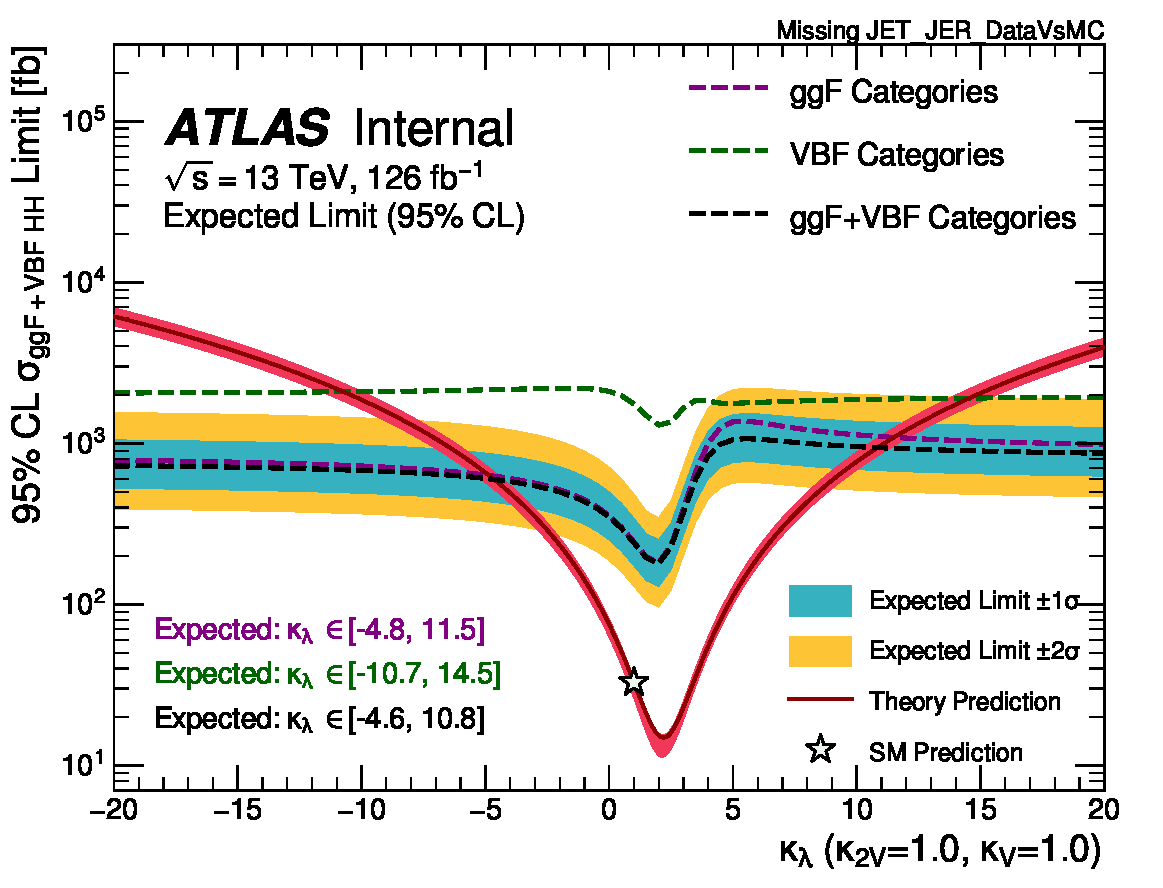
\includegraphics[width=0.45\textwidth]{\figDir/kl_scan_allcats_correlated_fullsyst_unblind_ggF_VBF_comb_samps_ggf_and_vbf_pd_ggf_161718_vbf_inc161718_k2v_1.0_xs.pdf}
	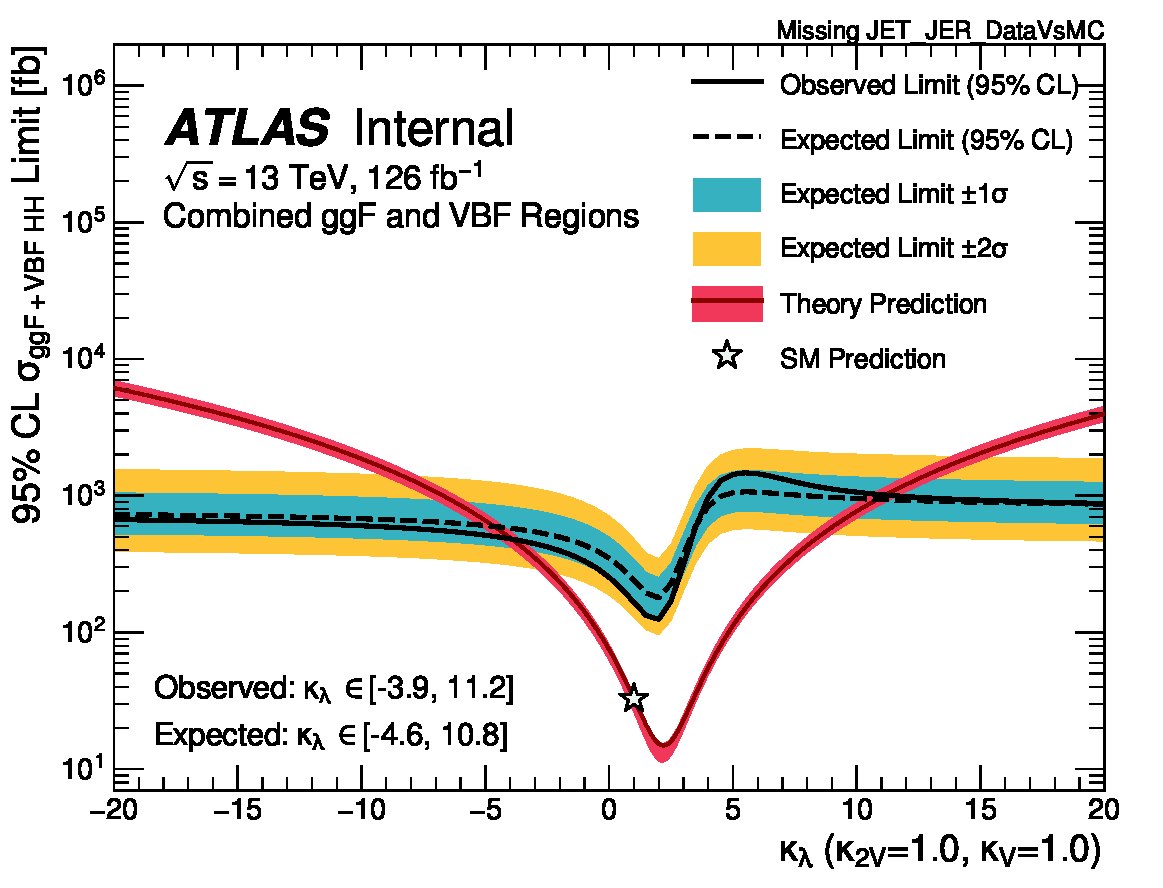
\includegraphics[width=0.45\textwidth]{\figDir/kl_scan_correlated_fullsyst_unblind_ggF_VBF_comb_samps_ggf_and_vbf_pd_ggf_161718_vbf_inc161718_k2v_1.0_xs.pdf} %{kl-scan-comb-uncorr-ratio-cats.pdf}
	\caption{The 95\% CLs limit on the combined ggF and VBF \HH production cross-sections.
	Left plot is a breakdown of channels.
	% , with the individual limits from the ggF (orange) and VBF (purple) channels overlaid.
	}
	\label{fig:comb_kl_scan}
\end{figure}

% \begin{figure}[h]
% 	\centering
% 	\subfloat[]{
% 		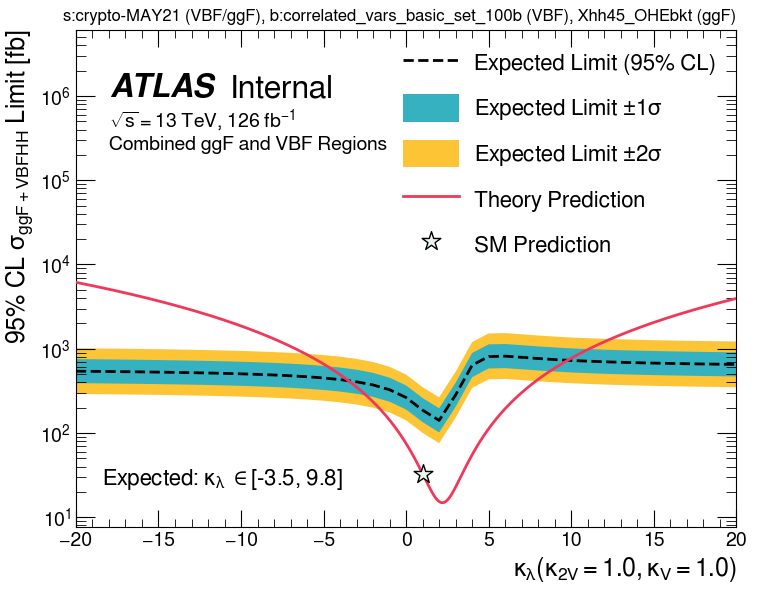
\includegraphics[width=0.48\textwidth]{xs_limit_plot_kl_ggf_and_vbf_all_yrs_FixedLumiNP.png}
% 		\label{fig:comb_kl_scan_a}
% 	}
% 	\subfloat[]{
% 		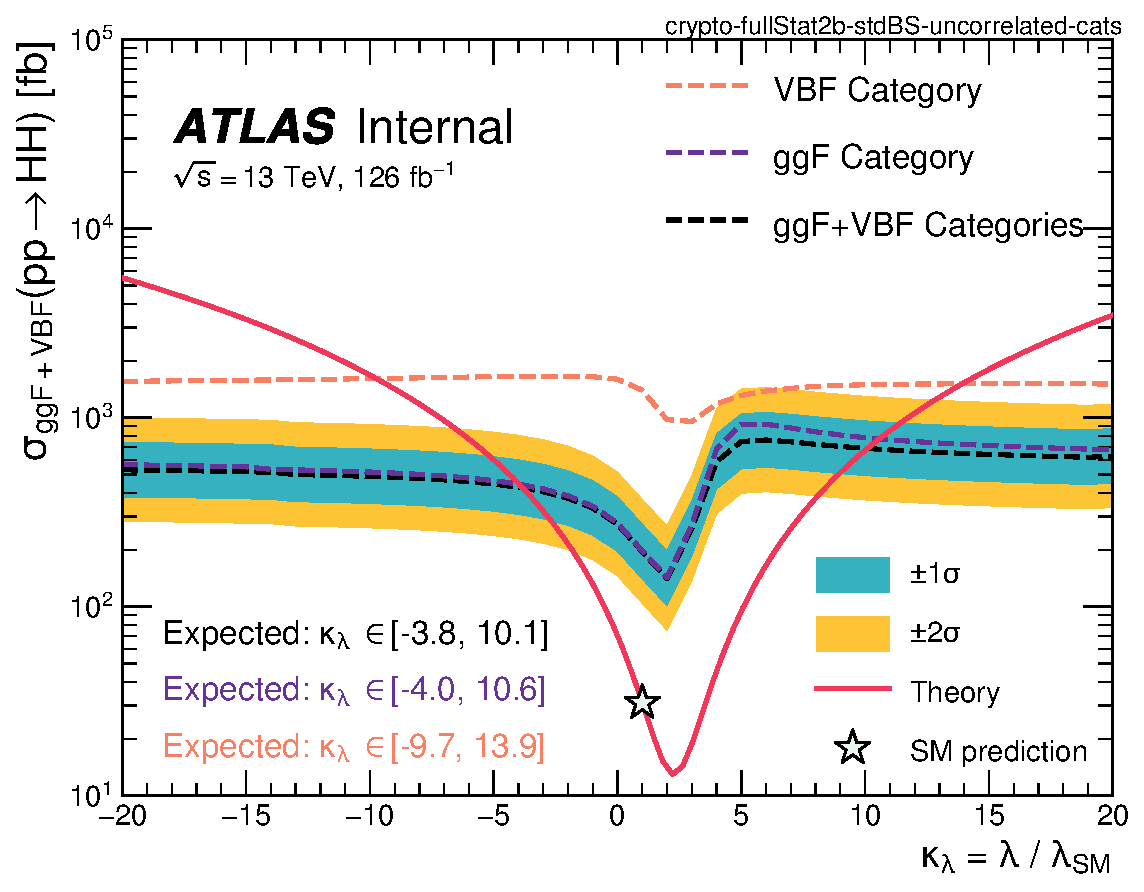
\includegraphics[width=0.48\textwidth]{kl-scan-comb-uncorr-ratio-cats.pdf}
% 		\label{fig:comb_kl_scan_b}
% 	}
% 	\caption{Figure \ref{fig:comb_kl_scan_a} shows the expected 95\% CLs limit on the combined ggF and VBF HH production cross-sections. Figure \ref{fig:comb_kl_scan_b} is identical to the previous Figure, but with the individual limits from the ggF (orange) and VBF (purple) channels overlaid.}
% 	\label{fig:comb_kl_scan}
% \end{figure}

\begin{table}[h]
	\centering
	\caption{In the combined channel, the observed and expected limit intervals on the coupling modifier \kl at the 95\% CL for the ggF channel, the VBF channel and the combination of the two.}
	\begin{tabular}{c c c}
		\toprule
		{Channel} & {Observed Interval} & {Expected Interval} \\
		\midrule
		{ggF Channel (ggF signal only)} & {$[-4.5, 13.3]$} & {$[-5.0, 12.0]$}  \\
		{VBF Channel (VBF signal only)}  & {$[-10.0, 13.2]$} & {$[-12.3, 15.6]$} \\
		{Combination (ggF+VBF signals)} & {$[-3.9, 11.2]$} & {$[-4.6, 10.8]$}  \\
		\bottomrule
	\end{tabular}
\label{table:kl-chan-comp-tab}
\end{table}

The scan for \kvv for the VBF production, but combining the ggF and VBF channels is shown in \Fig{\ref{fig:k2v-comb}}.
The ggF production is accounted for as a (very sub-dominant) background process, and the limit is set on the VBF signal production.
However, due to additional contributions of VBF events in the ggF SR, the expected constraint on \kvv [-0.05, 2.12] is slightly tighter than the VBF channel only constraint of [-0.08, 2.16].

\begin{figure}[ht]
	\centering
	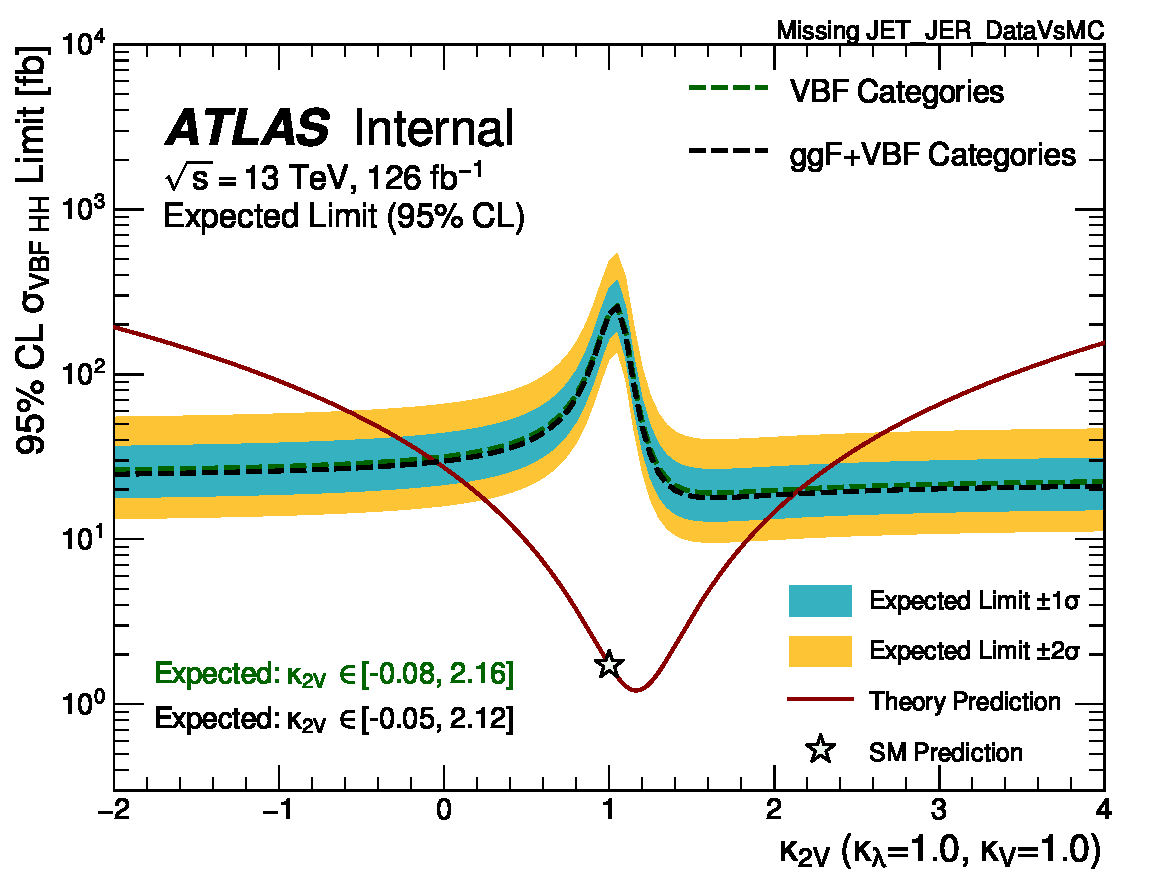
\includegraphics[width=0.45\textwidth]{\figDir/k2v_scan_allcats_correlated_fullsyst_unblind_ggF_VBF_comb_k2v_samps_ggf_and_vbf_pd_ggf_161718_vbf_inc161718_kl_1.0_xs.pdf}
	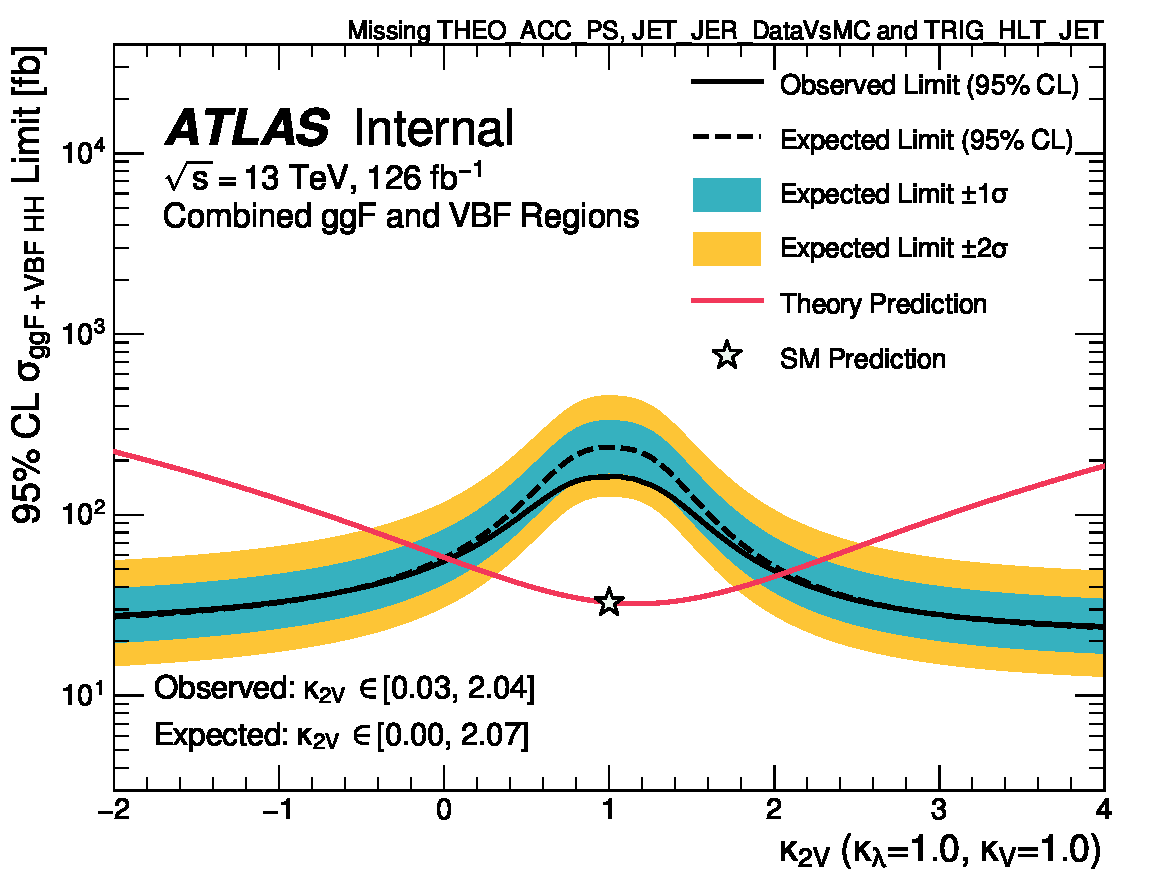
\includegraphics[width=0.45\textwidth]{\figDir/k2v_scan_correlated_fullsyst_unblind_ggF_VBF_comb_k2v_samps_ggf_and_vbf_pd_ggf_161718_vbf_inc161718_kl_1.0_xs.pdf}
	\caption{The limit intervals on the coupling modifier \kvv at the 95\% CL for the combination of the VBF+ggF channels.
	Left plot is a breakdown of channels.
	}
	\label{fig:k2v-comb}
\end{figure}

The 2D limit on the \kvv and \kl variations for the combined ggF + VBF channels is shown in \Fig{\ref{fig:2d-lim}} assuming $\kv = 1$.
Limits are derived from the intersection of the cross section limit and the theory predictions at given point.

\begin{figure}[ht]
	\centering
	\subfloat[]{
		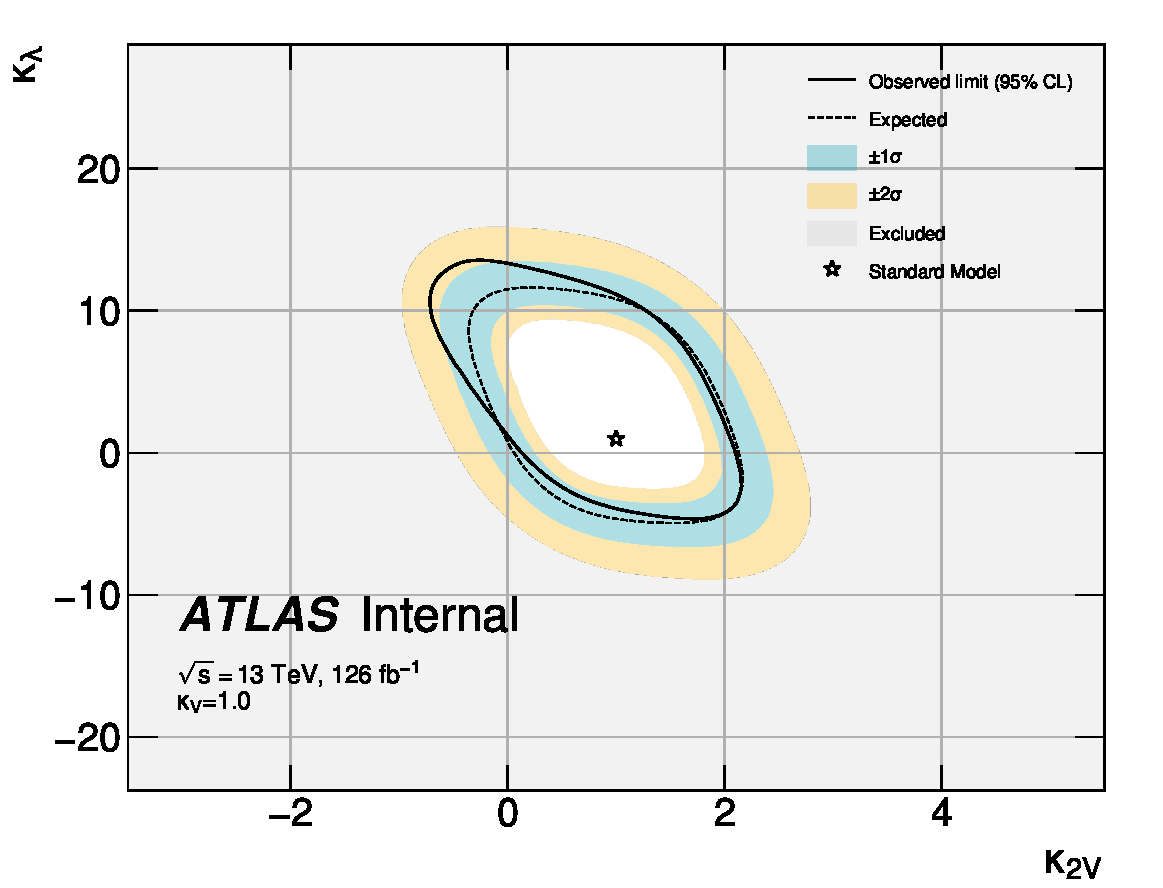
\includegraphics[width=0.44\textwidth]{\figDir/2D_scan_ggF_VBF_comb_samps_ggf_and_vbf_pd_ggf_161718_vbf_inc161718_k1v1.0_exclusion.pdf}
	}
	\subfloat[]{
		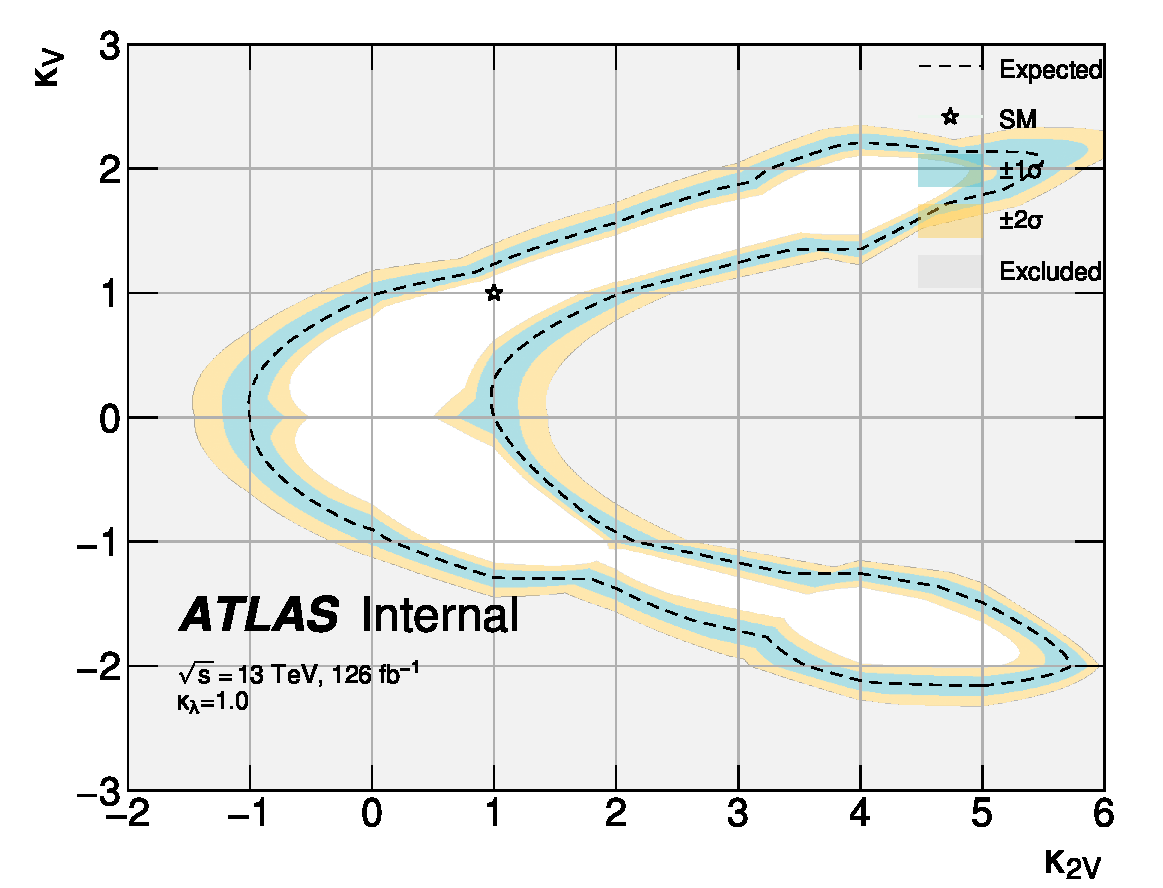
\includegraphics[width=0.44\textwidth]{figures/nr-int-note/results/V3/2D_scan_cmilke_full_3D_wide_scan_comb_samps_ggf_and_vbf_pd_ggf_161718_vbf_inc161718_kl1p0_exclusion.pdf}
	}
	\caption{The obs (solid) and expected (dashed) limit intervals on the coupling modifiers \kl vs \kvv (a) and \kv vs \kvv (b) at the 95\% CL for the combination of the VBF+ggF channels.
	\todo{(b) is expected only and with only the background shape uncertainties included. To be updated.}}
	\label{fig:2d-lim}
\end{figure}

\subsection{Improvements from previous analyses}

\textbf{To do: Make the history of the analysis plot!!}

\textbf{To do: Remake the cat improvements plots!!}

% To demonstrate the expected improved sensitivity from the addition of the \deta and \Xhh categories, a comparison of the SM signal limits with and without these categories is shown in \Fig{\ref{fig:sm-limit}} on the pre-fit Asimov dataset with background CR12 shape uncertainties only and with the decorrelated scheme.
% The categorization gives us a $\sim$30\% improvement in the SM limits. 
% \Fig{\ref{fig:kl-scan-ratio}} shows the corresponding \kl scan and the corresponding increase in sensitivity from the categorization.\footnote{For these limits, finer \mhh binning in the \mhh inclusive fit is used to maintain a similar number of bins with and without categorization.}

% \begin{figure}[ht]
% 	\centering
% 	\subfloat[]
% 	{
% 	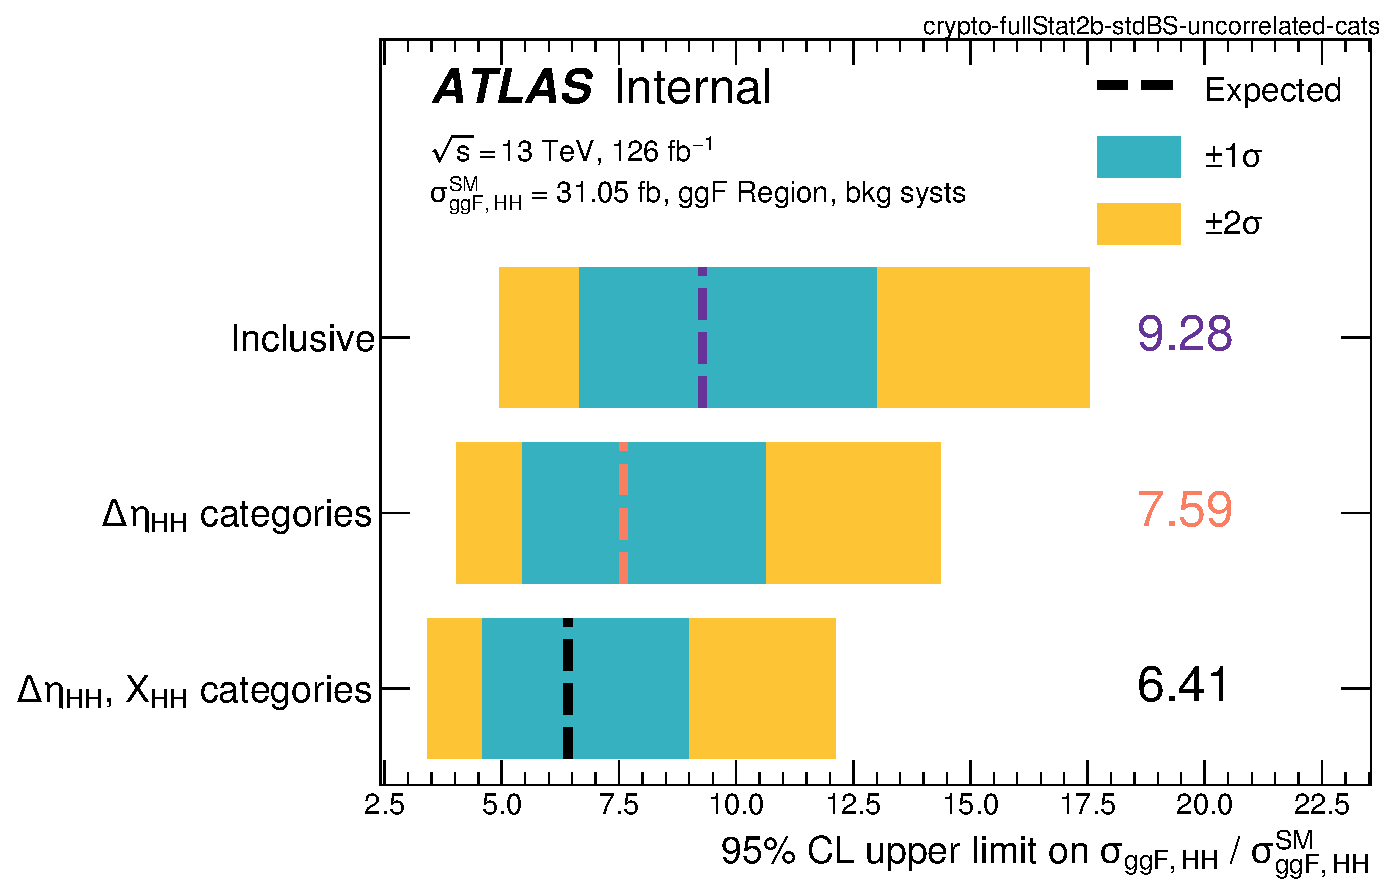
\includegraphics[width=0.44\textwidth]{sm-lim-uncorr}
% 	\label{fig:sm-limit}
% 	}
% 	\subfloat[]
% 	{
% 		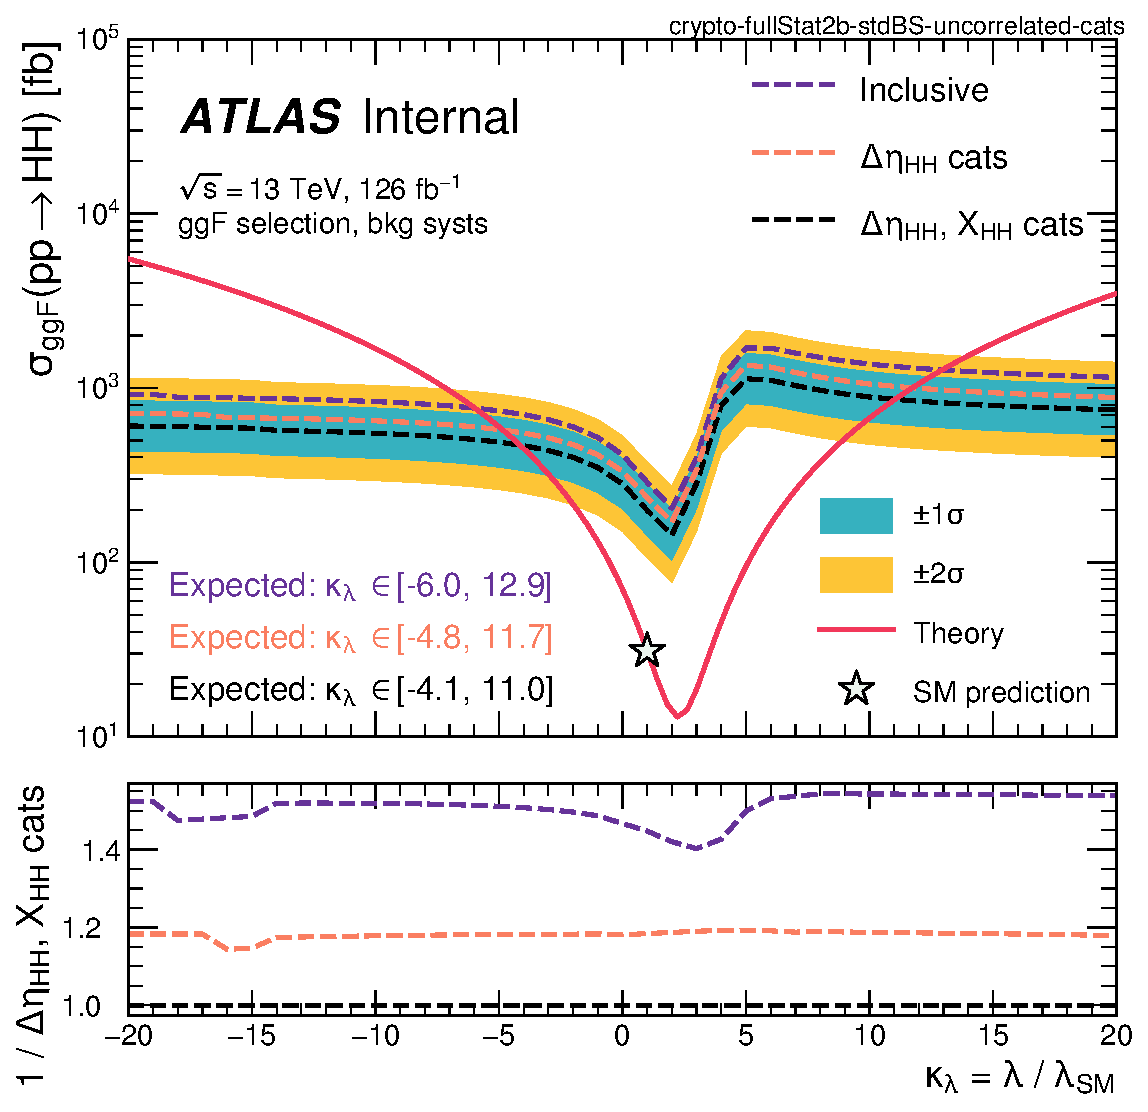
\includegraphics[width=0.5\textwidth]{kl-scan-uncorr-ratio-cats}
% 		\label{fig:kl-scan-ratio}
% 	}
% 	\caption{Expected sensitivity improvements for the ggF analysis by categorizing the fit discriminant (progressively adding \deta only, then the \Xhh categories).
% 	Studies are done on pre-fit Asimov with bkg-only systematics uncorrelated.
% 	 }
% 	\label{fig:ggF-ratio}
% \end{figure}